\documentclass{article} % For LaTeX2e
\usepackage{nips15submit_e,times}
\usepackage{hyperref}
\usepackage{url}
\usepackage{amsmath}
\usepackage{amsfonts}
\usepackage{amssymb}
\usepackage{amsthm}
\usepackage{natbib}
\usepackage{graphicx}
%\documentstyle[nips14submit_09,times,art10]{article} % For LaTeX 2.09


\title{What If Without the Conformal Prediction Method}


\author{
XIONG Zhixi\\
Department of Mathematics\\
Hong Kong University of Science and Technology\\
Hong Kong, China
}

% The \author macro works with any number of authors. There are two commands
% used to separate the names and addresses of multiple authors: \And and \AND.
%
% Using \And between authors leaves it to \LaTeX{} to determine where to break
% the lines. Using \AND forces a linebreak at that point. So, if \LaTeX{}
% puts 3 of 4 authors names on the first line, and the last on the second
% line, try using \AND instead of \And before the third author name.

\newcommand{\fix}{\marginpar{FIX}}
\newcommand{\new}{\marginpar{NEW}}

\nipsfinalcopy % Uncomment for camera-ready version

\begin{document}


\maketitle

\begin{abstract}
Reliable uncertainty quantification (UQ) is essential for deploying machine learning models in high-stakes domains such as medical diagnosis and autonomous systems.
However, traditional UQ methods often rely on strong distributional assumptions or asymptotic approximations that fail in finite-sample regimes.
This paper investigates Conformal Prediction (CP) as a model-agnostic and distribution-free framework that provides rigorous safety guarantees.
To handle complex data characteristics, we explore advanced variants, specifically Conformalized Quantile Regression (CQR), Weighted Conformal Prediction (WCP), and Mondrian Conformal Prediction (MCP), to address challenges regarding heteroscedasticity, covariate shift, and conditional coverage.
Through comparative experiments on synthetic non-Gaussian data and real-world benchmarks, we demonstrate that CP effectively calibrates the outputs of diverse black-box predictors, ranging from linear regression to deep neural networks, ensuring user-specified coverage rates where baselines like Monte Carlo (MC) Dropout and parametric methods frequently fail to meet the target coverage.
Our results highlight CP as a necessary ``safety wrapper'' that transforms arbitrary predictive models into trustworthy decision-making tools without sacrificing predictive efficiency. The code are available at \url{https://github.com/Leroy-Xiong/conformal_prediction}.
\end{abstract}

\section{Introduction}

In scientific, engineering, and everyday decision-making, obtaining a prediction is insufficient without also understanding its reliability through effective uncertainty quantification (UQ). Whether in autonomous driving, medical diagnosis, or financial risk assessment, relying solely on point estimates poses significant risks, as models are always imperfect and the world exhibits inherent noise. This challenge is formalized in classical decision theory, where optimal decisions require not only an expected outcome but a complete characterization of uncertainty. Formally, consider a decision problem where we observe data $x \in \mathcal{X}$ and must choose an action $a \in \mathcal{A}$. The consequence of this action depends on an unknown state $y \in \mathcal{Y}$, and is quantified by a loss function $L: \mathcal{A} \times \mathcal{Y} \to \mathbb{R}$. In the Bayesian decision theory \citep{berger1985statistical}, the optimal decision minimizes the \emph{posterior expected loss}:
\begin{equation}
    a^*(x) = \arg\min_{a \in \mathcal{A}} \mathbb{E}_{y \sim p(y|x)} \left[ L(a, y) \right] = \arg\min_{a \in \mathcal{A}} \int_{\mathcal{Y}} L(a, y) \, p(y|x) \, dy,
    \label{eq:bayesian_decision}
\end{equation}
where $p(y|x)$ is the posterior distribution of $y$ given $x$. As shown in (\ref{eq:bayesian_decision}), the optimal action $a^*$ depends not merely on a point estimate (such as the posterior mean), but on the entire posterior distribution. A poor characterization of $p(y|x)$ can lead to suboptimal decisions even with an accurate predictive model. Thus, robust and interpretable decision-making fundamentally requires well-calibrated uncertainty estimates. Consequently, a central challenge in modern machine learning, particularly for complex black-box models like deep neural networks, is to provide rigorous and reliable uncertainty measures for predictions. Without such measures, deploying these models in high-stakes domains remains risky.


To address this challenge, a variety of UQ methods have been developed, each with its own set of limitations that restrict practical applicability. Parametric models, for instance, often rely on strong distributional assumptions (e.g., normality) that are rarely justified in complex, real-world data settings \citep{wasserman2004all}. 
Asymptotic theories, while providing theoretical guarantees under ideal conditions, require sample sizes that are often unattainable in practice, and their convergence may not be guaranteed for finite or moderate datasets \citep{vovk2005algorithmic}. 
Within the Bayesian paradigm, the choice of a prior distribution can be subjective and difficult to justify. Furthermore, computing the posterior distribution is often intractable for high-dimensional or non-conjugate models, which often necessitates the use of approximate inference schemes that may themselves introduce errors \citep{murphy2012machine}.
Among more recent machine learning approaches, ensemble methods (e.g., deep ensembles \citep{lakshminarayanan2017simple}) can yield well-calibrated uncertainty estimates but at a prohibitive computational cost, as they require training and maintaining multiple models, which is a significant burden for large datasets and complex architectures. 
Techniques like Monte Carlo (MC) Dropout \citep{gal2016dropout} offer a more lightweight alternative by approximating Bayesian inference within neural networks, yet they impose specific architectural constraints (e.g., dropout layers) and require careful tuning of key hyperparameters, most notably the dropout rate, as well as the overall training schedule.
Lastly, generative models (e.g., diffusion \citep{ho2020denoising} or flow matching \citep{lipman2022flow}) can model complex data distributions but are notoriously expensive to train and may be challenging to scale to high-dimensional problems.
In summary, existing methods are often constrained by strong assumptions, high computational demands, or a lack of finite-sample guarantees, highlighting the need for a framework that is both model-agnostic and theoretically rigorous.

The conformal prediction (CP) framework emerges as a compelling solution to these limitations, offering a model-agnostic approach to UQ with finite-sample, distribution-free guarantees \citep{LearningByTransduction, vovk2005algorithmic}. Its core mechanism relies on the concept of \emph{nonconformity scores}. For any new input, CP evaluates how nonconforming each potential output appears relative to a set of labeled reference (or calibration) data. By calibrating a threshold based on the empirical distribution of these scores, CP constructs a prediction set (for classification) or a prediction interval (for regression) that is guaranteed to contain the true outcome with a user-specified probability (e.g., 90\%), under the weak assumption of data exchangeability. This procedure essentially uses past empirical errors to quantify future uncertainty, requiring no strong distributional assumptions, no modifications to the underlying model, and no asymptotic approximations.


Originally introduced by Gammerman, Vovk, and Vapnik in 1998 for Support Vector Machines, CP has transcended its initial scope to become a pervasive framework in modern reliable AI\@.
While theoretically grounded, its value is most evident in its rapidly expanding real-world impact across diverse high-stakes domains.
In the natural sciences, CP is now pivotal for guiding protein design sequences \citep{fannjiang2022conformal}.
In the realm of robotics and embodied AI, it facilitates safe planning in dynamic environments \citep{lindemann2023safe} and has been successfully applied to align uncertainty in Large Language Models (LLMs) for robotic interaction \citep{ren2023robots}.
The framework's reliability is equally critical in healthcare, where it has been deployed for estimating diagnostic uncertainty in cancer pathology \citep{olsson2022estimating} and predicting disease courses for conditions such as multiple sclerosis \citep{sreenivasan2025conformal}.
Additionally, CP has found utility in earth observation \citep{singh2024uncertainty}, further demonstrating its versatility and robustness in securing trust for safety-critical applications.
Collectively, these advancements illustrate the transformative potential of CP in bridging the gap between complex, black-box algorithms and the rigorous safety standards demanded by real-world applications.


\section{Methods}
\label{sec:methods}

This section formalizes the CP framework. We begin with the general transductive formulation, proceed to the computationally efficient Split Conformal Prediction (SCP), and conclude by discussing advanced variants designed to address limitations regarding adaptivity, distribution shifts, and conditional coverage.

\subsection{General Conformal Prediction Framework}

Consider a regression or classification problem where we observe a sequence of data points $Z_1, \dots, Z_n$, where $Z_i = (X_i, Y_i) \in \mathcal{X} \times \mathcal{Y}$. We assume these data points are \emph{exchangeable}, meaning their joint distribution is invariant under any permutation. Given a new test input $X_{n+1}$, our goal is to construct a prediction set $C(X_{n+1}) \subseteq \mathcal{Y}$ that covers the unknown true label $Y_{n+1}$ with a user-specified probability $1-\alpha$, where $\alpha \in (0, 1)$ is the miscoverage rate.

The general CP framework, often referred to as Full or Transductive CP \citep{vovk2005algorithmic}, relies on a \emph{nonconformity measure} $S: \mathcal{Z} \to \mathbb{R}$. This function assigns a score $s_i = S(Z_i)$ representing how ``unusual'' a data point $Z_i$ is relative to the others. 
For a candidate label $y \in \mathcal{Y}$ paired with $X_{n+1}$, we form a hypothetical dataset including $Z_{n+1} = (X_{n+1}, y)$. We then compute nonconformity scores for all $i \in \{1, \dots, n+1\}$. A $p$-value for the candidate $y$ is derived by comparing its score to the scores of the existing data:
\begin{equation}
    \pi(y) = \frac{1}{n+1} \sum_{i=1}^{n+1} \mathbb{I}\left( s_i \geq s_{n+1} \right),
    \label{eq:p_value}
\end{equation}
where $\mathbb{I}(\cdot)$ is the indicator function. The prediction set is constructed by including all candidates $y$ that appear statistically plausible:
\begin{equation}
    C_{\text{Full}}(X_{n+1}) = \left\{ y \in \mathcal{Y} \mid \pi(y) > \alpha \right\}.
    \label{eq:full_cp_set}
\end{equation}
Under the exchangeability assumption, this set satisfies the marginal validity property:
\begin{equation}
\mathbb{P}(Y_{n+1} \in C_{\text{Full}}(X_{n+1})) \ge 1-\alpha,
\end{equation}
for any sample size $n$ and any underlying distribution. The structure of the set $C_{\text{Full}}(X_{n+1})$ depends on the nature of the output space $\mathcal{Y}$:

\paragraph{Classification.} When $\mathcal{Y}$ is a finite set of discrete labels (e.g., $\{1, \dots, K\}$), we can explicitly calculate $\pi(y)$ for each possible class. The prediction set is simply the subset of labels for which the $p$-value exceeds $\alpha$.

\paragraph{Regression.} When $\mathcal{Y} = \mathbb{R}$, iterating through all possible values of $y$ is computationally impossible. However, for standard nonconformity measures (such as the absolute error $|y - \hat{\mu}(X_{n+1})|$), the function $\pi(y)$ is generally quasi-concave with respect to $y$. Consequently, the set defined in (\ref{eq:full_cp_set}) typically forms a continuous interval (or a union of intervals). In practice, this interval is computed by inverting the nonconformity score function to find the boundaries of $y$ that satisfy the condition $\pi(y) > \alpha$.

\subsection{Split Conformal Prediction}

While theoretically robust, Full CP is computationally prohibitive for complex models (e.g., neural networks) because it requires retraining the underlying model for every candidate $y$ to compute the scores $s_i$ properly. To address this computational bottleneck, SCP, also known as Inductive CP, is the most widely adopted variant in modern machine learning \citep{papadopoulos2002inductive, lei2018distribution}.

In SCP, the available data is partitioned into two disjoint subsets: a proper training set $\mathcal{D}_{\text{train}}$ and a calibration set $\mathcal{D}_{\text{cal}} = \{(X_i, Y_i)\}_{i=1}^{n}$. A predictive model is trained solely on $\mathcal{D}_{\text{train}}$. We then compute nonconformity scores on $\mathcal{D}_{\text{cal}}$ using this fixed model. The construction of the prediction set depends on the task type:

\paragraph{Classification.}
For a classification task with discrete labels $\mathcal{Y} = \{1, \dots, K\}$, the model $\hat{f}: \mathcal{X} \to [0, 1]^K$ typically outputs a probability distribution over classes, where $\hat{f}(x)_k$ denotes the estimated probability of class $k$. A common nonconformity score is the complement of the probability assigned to the true class:
\begin{equation}
    s_i = 1 - \hat{f}(X_i)_{Y_i}, \quad \forall i \in \mathcal{D}_{\text{cal}}.
\end{equation}
Let $\hat{q}$ be the $\lceil (n+1)(1-\alpha) \rceil / n$ empirical quantile of the calibration scores $\{s_1, \dots, s_n\}$. The prediction set includes all classes with a predicted probability above the calibrated threshold:
\begin{equation}
    C_{\text{SCP}}(X_{n+1}) = \left\{ k \in \mathcal{Y} \mid \hat{f}(X_{n+1})_k \ge 1 - \hat{q} \right\}.
    \label{eq:scp_set_class}
\end{equation}
This formulation, often referred to as Least Ambiguous Set-valued Classifiers \citep{sadinle2019least}, guarantees that the true label is included in the set with probability at least $1-\alpha$.

\paragraph{Regression.}
For a regression task ($\mathcal{Y} = \mathbb{R}$), let $\hat{\mu}: \mathcal{X} \to \mathbb{R}$ be the trained model. A standard choice for the nonconformity score is the absolute residual:
\begin{equation}
    s_i = |Y_i - \hat{\mu}(X_i)|, \quad \forall i \in \mathcal{D}_{\text{cal}}.
\end{equation}
Similarly, let $\hat{q}$ be the $\lceil (n+1)(1-\alpha) \rceil / n$ empirical quantile of these regression scores. The prediction set for a new input $X_{n+1}$ is constructed as a fixed-width interval:
\begin{equation}
    C_{\text{SCP}}(X_{n+1}) = \left[ \hat{\mu}(X_{n+1}) - \hat{q}, \quad \hat{\mu}(X_{n+1}) + \hat{q} \right].
    \label{eq:scp_interval}
\end{equation}

\vspace{0.5em}
In both cases, SCP maintains the finite-sample validity guarantee provided the calibration and test data are exchangeable. Because the model is trained only once, SCP is computationally efficient and model-agnostic.

\subsection{Advanced Variants addressing Limitations}

While SCP establishes a rigorous baseline for UQ, its standard formulation exhibits three significant limitations when applied to complex, real-world scenarios. First, the reliance on a global threshold produces prediction sets of fixed size (e.g., fixed-width intervals), failing to account for \emph{heteroscedasticity} where uncertainty varies locally across the input space. Second, the theoretical validity of SCP hinges on the assumption of exchangeability, which is often violated under \emph{covariate shifts} (e.g., distribution shift). Third, SCP only guarantees \emph{marginal} coverage averaged over the entire population, which permits systematic under-coverage for specific subgroups or minority classes. To address these challenges, several specialized variants have been developed.

\paragraph{Heteroscedasticity and Locally Adaptive Conformal Prediction.}
Standard SCP constructs prediction intervals of fixed width $2\hat{q}$ across the entire input space. This approach assumes homoscedasticity and results in inefficiency: the intervals are unnecessarily wide for ``easy'' inputs and potentially too narrow for ``hard'' ones. To address this, Conformalized Quantile Regression (CQR) \citep{romano2019conformal} was proposed to construct intervals that adapt their width to the local difficulty of the input. The CQR procedure consists of two main steps: Quantile Regression (QR) training and conformal calibration.

First, using the training set $\mathcal{D}_{\text{train}}$, we train a regression model $\hat{f}$ to estimate two conditional quantiles: the lower quantile at level $\gamma_{\text{lo}} = \alpha/2$ and the upper quantile at level $\gamma_{\text{hi}} = 1 - \alpha/2$. The model outputs $\hat{q}_{\text{lo}}(x)$ and $\hat{q}_{\text{hi}}(x)$, which are optimized by minimizing the pinball loss (or quantile loss) \citep{koenker2001quantile}:
\begin{equation}
    \mathcal{L}(y, \hat{y}, \gamma) = \max \left( \gamma (y - \hat{y}), (\gamma - 1) (y - \hat{y}) \right).
\end{equation}
The total objective minimizes the average loss over both quantiles: $\sum_{i \in \mathcal{D}_{\text{train}}} [\mathcal{L}(y_i, \hat{q}_{\text{lo}}(x_i), \gamma_{\text{lo}}) + \mathcal{L}(y_i, \hat{q}_{\text{hi}}(x_i), \gamma_{\text{hi}})]$.

Second, although these raw quantile estimates provide a heuristic interval $[\hat{q}_{\text{lo}}(X), \hat{q}_{\text{hi}}(X)]$, they do not guarantee finite-sample coverage. CQR acts as a ``wrapper'' to rigorously calibrate them. We compute nonconformity scores on the calibration set $\mathcal{D}_{\text{cal}}$ as:
\begin{equation}
    s_i = \max \left( \hat{q}_{\text{lo}}(X_i) - Y_i, \; Y_i - \hat{q}_{\text{hi}}(X_i) \right).
\end{equation}
Intuitively, $s_i$ measures the signed distance from the true label $Y_i$ to the nearest boundary of the predicted interval. If $Y_i$ falls inside the interval, $s_i$ is negative; if it falls outside, $s_i$ is positive.

Let $\hat{q}$ be the $\lceil (n+1)(1-\alpha) \rceil / n$ empirical quantile of these scores $\{s_1, \dots, s_n\}$. The final conformalized prediction interval for a new input $X_{n+1}$ is constructed by expanding (or shrinking) the raw quantile estimates by $\hat{q}$:
\begin{equation}
    C_{\text{CQR}}(X_{n+1}) = \left[ \hat{q}_{\text{lo}}(X_{n+1}) - \hat{q}, \quad \hat{q}_{\text{hi}}(X_{n+1}) + \hat{q} \right].
\end{equation}
This procedure ensures valid coverage while allowing the interval width $\hat{q}_{\text{hi}}(X) - \hat{q}_{\text{lo}}(X) + 2\hat{q}$ to vary dynamically based on the input $X$, significantly improving informativeness in heteroscedastic settings.

\paragraph{Covariate Shift and Weighted Conformal Prediction.}
The standard exchangeability assumption is violated under distribution shift, where the test distribution $P_{\text{test}}(X)$ differs from the training distribution $P_{\text{train}}(X)$. Under such \emph{covariate shift}, standard CP loses its coverage guarantee. \cite{tibshirani2019conformal} proposed \emph{Weighted Conformal Prediction} (WCP), which adjusts the quantile calculation using likelihood ratios. For each calibration point $X_i \in \mathcal{D}_{\text{cal}}$, we assign a weight proportional to the density ratio:
\begin{equation}
    w(X_i) = \frac{dP_{\text{test}}(X_i)}{dP_{\text{train}}(X_i)} = \frac{p_{\text{test}}(X_i)}{p_{\text{train}}(X_i)},
\end{equation}
where $p_{\text{test}}$ and $p_{\text{train}}$ denote the probability density functions (or probability mass functions) of the test and training distributions, respectively. Intuitively, $w(X_i)$ quantifies how much more likely the input $X_i$ is to appear in the test environment compared to the training environment.

Given these weights, WCP modifies the standard calibration procedure by replacing the uniform empirical distribution with a weighted counterpart. Specifically, after computing nonconformity scores $\{s_i\}_{i=1}^n$ on the calibration set, we assign a normalized probability mass to each point. For a new test input $X_{n+1}$, the calibration points are weighted by $w(X_i)$, while the test point itself is assigned a fixed weight of 1 (reflecting its draw from the target distribution). The resulting probability weights are defined as:
\begin{equation}
    p_i(X_{n+1}) = \frac{w(X_i)}{\sum_{j=1}^n w(X_j) + 1}, \quad p_{n+1}(X_{n+1}) = \frac{1}{\sum_{j=1}^n w(X_j) + 1}.
\end{equation}
These probabilities are then used to construct the weighted empirical cumulative distribution function of the scores:
\begin{equation}
    \hat{F}(s) = \sum_{i=1}^n p_i(X_{n+1}) \, \mathbb{I}(s_i \le s) + p_{n+1}(X_{n+1}) \, \mathbb{I}(\infty \le s).
\end{equation}
The calibrated threshold $\hat{q}$ is determined as the smallest score $s$ such that $\hat{F}(s) \ge 1-\alpha$. Consequently, the final prediction set is formed as $C_{\text{WCP}}(X_{n+1}) = [\hat{\mu}(X_{n+1}) - \hat{q}, \; \hat{\mu}(X_{n+1}) + \hat{q}]$. By incorporating the likelihood ratio into the quantile estimation, this method ensures that the coverage guarantee holds with respect to the target distribution $P_{\text{test}}$.

\paragraph{Conditional Coverage and Mondrian Conformal Prediction.}
Standard SCP guarantees \emph{marginal} coverage, meaning $\mathbb{P}(Y \in C(X)) \ge 1-\alpha$ on average over the entire population. However, this global guarantee allows for systematic under-coverage in specific subgroups (e.g., minority classes or difficult input regions) as long as it is compensated by over-coverage elsewhere. To address this, Mondrian Conformal Prediction (MCP) \citep{vovk2005algorithmic} enforces validity within defined categories.

Let $K: \mathcal{X} \to \{1, \dots, M\}$ be a taxonomy function that maps an input $X$ to one of $M$ categories (or ``bins''). We partition the calibration set $\mathcal{D}_{\text{cal}}$ into disjoint subsets based on these categories:
\begin{equation}
    \mathcal{D}_{\text{cal}}^{(m)} = \{ (X_i, Y_i) \in \mathcal{D}_{\text{cal}} \mid K(X_i) = m \}, \quad \text{for } m = 1, \dots, M.
\end{equation}
Calibration is then performed independently within each bin. For a new test input $X_{n+1}$ belonging to category $m^* = K(X_{n+1})$, we compute the nonconformity scores using only the data in $\mathcal{D}_{\text{cal}}^{(m^*)}$. Let $n_{m^*} = |\mathcal{D}_{\text{cal}}^{(m^*)}|$ be the number of calibration samples in this category. We calculate the category-specific quantile $\hat{q}_{1-\alpha}^{(m^*)}$ as the $\lceil (n_{m^*} + 1)(1-\alpha) \rceil / n_{m^*}$ empirical quantile of the scores in $\mathcal{D}_{\text{cal}}^{(m^*)}$. The prediction set is then constructed as:
\begin{equation}
    C_{\text{MCP}}(X_{n+1}) = \left\{ y \in \mathcal{Y} \mid S((X_{n+1}, y)) \le \hat{q}_{1-\alpha}^{(m^*)} \right\}.
\end{equation}
By stratifying the calibration process, MCP ensures that the coverage guarantee holds conditionally for each group:
\begin{equation}
    \mathbb{P}(Y_{n+1} \in C_{\text{MCP}}(X_{n+1}) \mid K(X_{n+1}) = m) \ge 1-\alpha, \quad \forall m \in \{1, \dots, M\}.
\end{equation}
This property is particularly vital in safety-critical applications where fairness across subgroups or reliability across different operating modes is required.


\section{Advantages and Impact}

The CP framework offers a rigorous alternative to traditional UQ methods. Its rising popularity in statistical machine learning is driven by several distinctive advantages that address the limitations of parametric and asymptotic approaches.

\subsection{Finite-Sample Coverage}
A defining characteristic of CP is its validity for any finite sample size $n$. Unlike asymptotic statistical theories, which guarantee coverage only as $n \to \infty$, CP ensures that the constructed prediction sets cover the true outcome with probability at least $1-\alpha$ even when the number of available data points is small. This finite-sample validity is derived directly from the randomization of the data sequence and does not rely on large-sample approximations. This property is particularly vital in domains where data collection is expensive or scarce, ensuring that the reported confidence levels are trustworthy regardless of dataset size.

To empirically validate this theoretical guarantee, particularly in data-scarce regimes, we conducted a comparative experiment using the \textit{Diabetes} dataset. We employed Gradient Boosting QR as the base model to predict disease progression based on BMI and other features. The data was partitioned to simulate a small-sample setting with a calibration set of only $N_{\text{cal}}=50$ samples. We compared the raw output of the quantile regressors against the CQR method, targeting a 90\% coverage rate ($\alpha=0.1$).

\begin{figure}[htb!]
    \centering
    \includegraphics[width=\linewidth]{figures/finite_sample_coverage.jpg}
    \caption{\textbf{Validation of Finite-Sample Guarantee on the Diabetes Dataset.} 
    \textbf{(a)} The distribution of the dataset (BMI vs. Target). 
    \textbf{(b)} A snapshot of a single trial comparing Raw QR bounds (red dashed lines) with CP intervals (green band). The yellow stars indicate test points that fell outside the raw model's bounds but were successfully captured by the CP correction ($\hat{q}$ adjustment).
    \textbf{(c)} Distribution of empirical coverage rates over 100 trials. The Raw QR method (red) consistently under-covers (mean $\approx$ 87.8\%), failing to meet the 90\% target (dashed line) due to finite-sample errors. In contrast, CQR (green) rigorously satisfies the validity property (mean $\approx$ 92.3\%).
    \textbf{(d)} The boxplot of interval widths shows that CP achieves validity by appropriately expanding the intervals to account for the uncertainty inherent in the small calibration set.}\label{fig:finite_sample_experiment}
\end{figure}

The results, visualized in Figure~\ref{fig:finite_sample_experiment}, clearly demonstrate the risks of relying on asymptotic approximations when sample sizes are finite. As shown in Panel (c), the raw QR (competitor) consistently fails to meet the user-specified 90\% confidence level, achieving an average coverage of only 87.8\%. This under-coverage occurs because the asymptotic assumptions of the quantile loss do not hold for $N_{\text{cal}}=50$.

In contrast, the CP method corrects these errors. By computing a calibrated adjustment factor $\hat{q}$ based on the empirical distribution of nonconformity scores, CP ensures the target coverage is met (average 92.3\%). Panel (b) illustrates the mechanism: the CP intervals (green band) dynamically expand beyond the raw model predictions (red dashed lines) to capture ``hard'' examples (marked with yellow stars), effectively acting as a safety net. While this correction results in slightly wider intervals (Panel d), it is a necessary trade-off to guarantee reliability in safety-critical or data-limited applications.

\subsection{Distribution-Free}
CP is inherently distribution-free, meaning its validity holds for any underlying joint distribution $P_{XY}$, provided the data points are exchangeable. Traditional parametric methods often rely on strong assumptions, such as the normality of error terms (Gaussianity), which are frequently violated in complex, real-world high-dimensional data. CP requires no knowledge of the generative process and no estimation of density functions. By relying solely on the exchangeability assumption (which is satisfied by i.i.d.\ data), CP remains robust even in the presence of heavy tails or skewness.

\begin{figure}[htb!]
    \centering
    \includegraphics[width=\textwidth]{figures/distribution_free.jpg} % Replace with your actual file name
    \caption{\textbf{Validation of Distribution-Free Robustness.}
    \textbf{(a)} Histogram of the actual residuals (blue) versus the Gaussian fit (red dashed line) assumed by the baseline method. The clear skewness and heavy tail of the actual data violate the normality assumption, leading to a poor fit.
    \textbf{(b)} Comparison of empirical coverage rates. The Gaussian baseline (yellow) fails to capture the true distribution's shape, resulting in unpredictable coverage. In contrast, CP (green) achieves near-perfect validity (90.8\%) by relying on the empirical quantiles of the residuals rather than a density estimate.
    \textbf{(c)} Visualization of CP intervals for the first 50 test samples. The intervals (green bars) effectively contain the true targets (black crosses) even in the presence of asymmetric noise, with failures (red crosses) occurring at the expected rate of $\alpha=10\%$.}\label{fig:dist_free_experiment}
\end{figure}

To demonstrate this robustness against non-standard distributions, we performed an experiment using synthetic data with explicitly non-Gaussian noise. We generated a non-linear regression dataset and added skewed noise drawn from an exponential distribution (centered to zero). This setup mimics real-world scenarios where error terms are asymmetric and heavy-tailed, violating the standard Gaussian assumption utilized by many parametric methods. We trained a neural network regressor and compared a baseline Gaussian uncertainty estimation (Mean $\pm 1.64\sigma$) against CP, both targeting a 90\% coverage rate.

The results, shown in Figure~\ref{fig:dist_free_experiment}, underscore the necessity of distribution-free methods. Panel (a) reveals the significant discrepancy between the actual skewed residuals (blue histogram) and the fitted Gaussian distribution (red dashed line). Because the baseline method assumes symmetry and thin tails, it cannot accurately model the risk. Consequently, as shown in Panel (b), the baseline achieves an arbitrary coverage rate that may not align with the safety requirement.

However, CP remains unaffected by the skewness. By computing the nonconformity scores directly from the data and determining the threshold empirically (Panel c), it achieves a coverage of 90.8\%, aligning almost perfectly with the target. This confirms that CP provides valid UQ for arbitrary data distributions without requiring feature engineering or complex density estimation.

\subsection{Model-Free}
The CP framework, particularly the Split CP formulation, is fully model-agnostic. It operates as a ``wrapper'' around any predictive model, decoupling the task of UQ from model training. Whether the underlying predictor is a simple linear regression or a massive deep neural network, CP can calibrate its outputs without requiring modifications to the model architecture, loss function, or optimization procedure. This contrasts significantly with Bayesian Neural Networks or Deep Ensembles, which often impose specific structural constraints or incur prohibitive computational costs. This flexibility allows researchers to equip state-of-the-art ``black-box'' models with rigorous uncertainty estimates efficiently.

\begin{figure}[htb!]
    \includegraphics[width=\textwidth]{figures/model_free.jpg} % Replace with your actual file name
    \caption{\textbf{Evaluation of Model Agnosticism across 7 Architectures.} 
    \textbf{(a)} Models sorted by predictive error (MSE), ranging from weaker models (KNN, Linear) to strong ensembles (Gradient Boosting).
    \textbf{(b)} The average prediction interval width follows the trend of the MSE\@. Stronger models like Gradient Boosting produce significantly sharper intervals (17.7 units) compared to the Linear baseline (37.5 units).
    \textbf{(c)} Empirical coverage rates for all models. Despite the vast differences in underlying mathematical principles and accuracy, CP ensures that every model approximates the 90\% target (dashed line), validating the model-free property.}\label{fig:model_free_results}
\end{figure}

To rigorously verify the model-agnostic property of the CP framework, we conducted a comprehensive experiment using the \textit{Concrete Compressive Strength} dataset. We employed seven distinct machine learning architectures spanning the major paradigms of regression: Instance-based (KNN), Linear (Ridge), Tree-based (Decision Tree), Kernel-based (SVR), Ensemble methods (Random Forest, Gradient Boosting), and Deep Learning (Neural Network). The target miscoverage rate was set to $\alpha=0.1$ (90\% confidence). 

First, validity is invariant to model choice. As shown in Panel (c), all seven models achieve empirical coverage rates close to the nominal 90\% level, regardless of whether the model is a simple linear equation or a complex non-linear ensemble. It is worth noting that some methods, such as the Decision Tree (88.0\%) or Random Forest (88.7\%), exhibit coverage slightly below the exact 90\% threshold. This does not indicate a failure of the method. The coverage guarantee provided by SCP is marginal ($1-\alpha$) over the randomness of the calibration/test split. For any finite test set size $N_{test}$, the observed coverage follows a binomial distribution around $1-\alpha$. Therefore, minor fluctuations (e.g., $\pm 2\%$) are expected statistical noise inherent to finite-sample evaluation, not a violation of the theoretical validity.

Second, accuracy translates to efficiency. Panels (a) and (b) demonstrate the clear advantage of using high-performance models. There is a clear correlation between the Mean Squared Error and the average interval width. The Gradient Boosting regressor, which achieves the lowest error (MSE $\approx$ 35), produces the sharpest uncertainty estimates with an average width of 17.7 units. In contrast, the Linear Ridge model (MSE $\approx$ 114) requires intervals more than twice as wide (37.5 units) to achieve the same 90\% safety guarantee. This confirms that while CP acts as a universal safety net, improving the underlying ``black-box'' model directly rewards the user with more informative and actionable prediction sets.

\vspace{0.5em}
Collectively, these advantages have positioned CP as a cornerstone of modern reliable AI\@. By providing a framework that is theoretically rigorous yet practically implementable, CP has bridged the gap between abstract statistical guarantees and high-stakes applications. It has enabled safe decision-making in fields such as medical diagnostics, where ``knowing what the model doesn't know'' is as critical as prediction accuracy. Furthermore, it has spurred a new direction of research focused on distribution shifts and fairness, ensuring that machine learning systems remain safe and robust in dynamic, open-world environments.


\section{Comparative Analysis}

To rigorously evaluate the practical advantages of CP over traditional and modern UQ paradigms, we conducted a comparative study using the \textit{California Housing} dataset. This real-world regression task features complex, non-linear dependencies and a skewed target distribution, serving as an ideal testbed to assess how different methods handle deviations from ideal theoretical assumptions.

\subsection{Experimental Setup and Baselines}
We evaluate the performance of each method using two complementary metrics: \textit{Empirical Coverage}, which measures the safety of the method (the proportion of test labels contained within the prediction intervals), and \textit{Average Interval Width}, which quantifies the efficiency (narrower intervals are more informative). The experiments were conducted with a target significance level of $\alpha=0.1$, corresponding to a 90\% confidence interval. We compared the SCP implementation (using an XGBoost base learner) against five representative competitors spanning the UQ landscape:

\begin{enumerate}
    \item \textbf{Parametric (Linear Regression):} Represents classical frequentist statistics. It constructs prediction intervals assuming the data follows a homoscedastic Gaussian distribution around a linear fit.
    \item \textbf{Bayesian (Bayesian Ridge):} Represents probabilistic modeling. It incorporates prior beliefs and quantifies uncertainty via the posterior predictive distribution, also assuming Gaussianity.
    \item \textbf{Ensemble (Random Forest):} A non-parametric machine learning approach that estimates uncertainty using the empirical variance of predictions across decision trees.
    \item \textbf{Quantile Regression (GBDT):} A direct estimation method that minimizes the pinball loss to predict the $\alpha/2$ and $1-\alpha/2$ conditional quantiles, theoretically asymptotically valid.
    \item \textbf{Monte Carlo (MC) Dropout:} A popular deep learning technique \citep{gal2016dropout} that approximates Bayesian inference by keeping dropout layers active during inference to capture model uncertainty.
\end{enumerate}

% FIGURE DEFINITION
\begin{figure}[htb!]
    \centering
    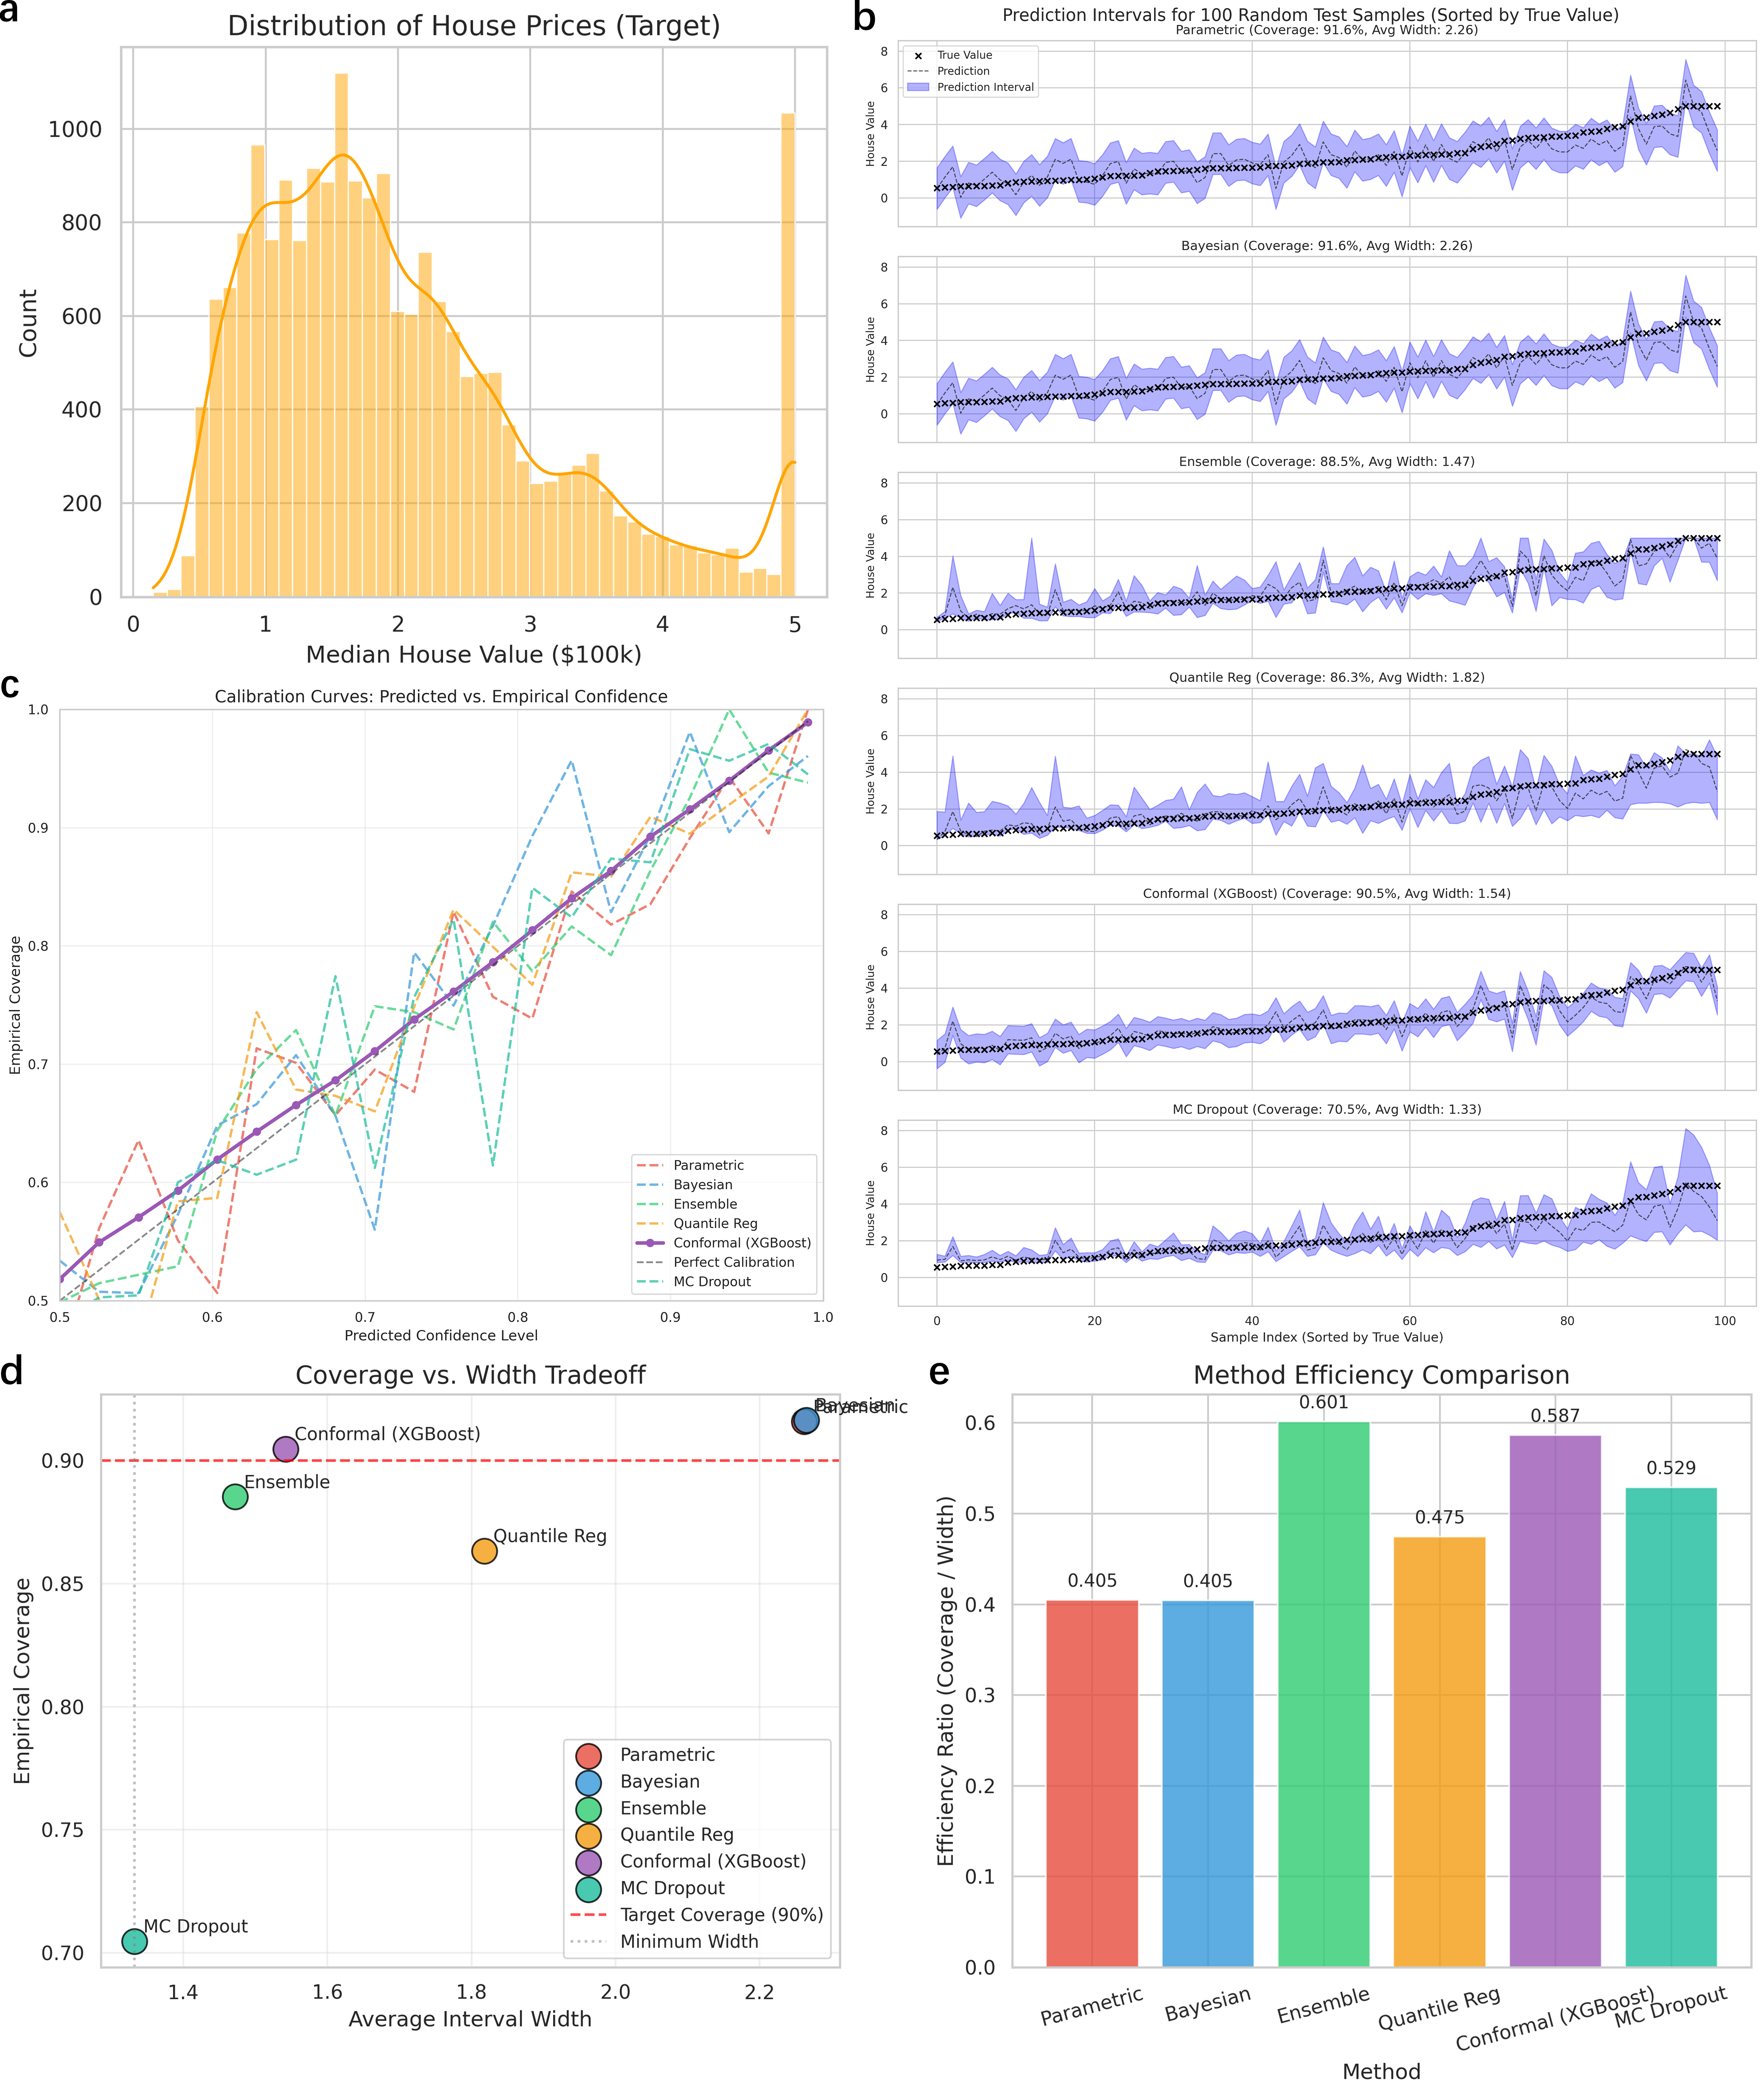
\includegraphics[width=1.0\textwidth]{figures/model_comparison.jpg} % Replace with your actual filename
    \caption{\textbf{Comparative Analysis of Uncertainty Quantification Methods on California Housing Data.} 
    \textbf{(a)} The target distribution (House Prices) is non-Gaussian, challenging parametric assumptions. 
    \textbf{(b)} Prediction intervals for random test samples. Parametric and Bayesian methods produce overly wide, uniform intervals. MC Dropout produces narrow intervals that fail to cover the true label (black crosses). CP produces adaptive, valid intervals.
    \textbf{(c)} Calibration curves showing Empirical Coverage vs. Predicted Confidence. CP (purple solid line) aligns closely with the ideal diagonal, indicating perfect calibration, while other methods indicate miscalibration.
    \textbf{(d)} Coverage-Width Trade-off. The red dashed line indicates the 90\% target. CP (purple dot) is the only method that meets the safety requirement (Coverage $\ge 90\%$) while maintaining low interval width.
    \textbf{(e)} Efficiency Ratio (Coverage/Width). While Ensembles are efficient, they lack the finite-sample guarantee of CP.}
    \label{fig:comparison_results}
\end{figure}


\subsection{Results and Discussion}

The experimental results, visualized in Figure~\ref{fig:comparison_results}, underscore the critical limitations of conventional UQ methods when faced with real-world data complexities. As illustrated in Panel (a), the distribution of house prices is highly non-Gaussian, a characteristic that directly challenges parametric and Bayesian approaches relying on normality assumptions. Consequently, these methods are forced to output excessively wide intervals (Average Width $\approx 2.26$, see Panel d) to accommodate the data's skewness. While they technically meet the validity requirement ($>91\%$ coverage), they do so inefficiently, offering coarse uncertainty estimates that provide little actionable information to the user.

Conversely, modern machine learning approaches that rely on asymptotic approximations struggle to maintain validity in finite-sample regimes. This is most evident in the performance of MC Dropout and QR\@. As shown in the bottom trace of Panel (b), MC Dropout drastically under-covers, achieving only 70.5\% coverage against the 90\% target. This creates a false sense of security, presenting narrow but unreliable intervals that are dangerous for safety-critical applications. Similarly, QR, despite being theoretically sound asymptotically, suffers from finite-sample variability in practice, reaching only 86.3\% coverage and failing to strictly meet the safety standard. Likewise, the Ensemble approach, while producing efficient intervals, achieved a coverage of 88.5\%, illustrating that empirical variance across decision trees serves as a practical approximation but lacks the formal coverage guarantees required for rigorous UQ.

The superior reliability of CP is further demonstrated by the calibration curves in Panel (c), where SCP (purple line) exhibits the tightest alignment with the ideal diagonal, contrasting sharply with the significant deviation of the competitors. This balance between safety and utility is summarized in the trade-off analysis in Panel (d). While parametric methods fall into the ``safe but inefficient'' region and MC Dropout into the ``efficient but unsafe'' region, CP strikes the optimal balance. By explicitly utilizing a calibration set to compute the exact empirical quantile adjustment, CP ensures the coverage guarantee (achieving 90.5\%) while maintaining sharp, informative intervals (Average Width $\approx 1.54$), significantly outperforming the uncalibrated baselines.

Ultimately, this comparative analysis confirms that while complex models like Neural Networks or Ensembles can learn high-performance point predictions, they do not inherently provide reliable uncertainty estimates. The CP framework acts as a necessary safety layer, effectively transforming the raw, often miscalibrated outputs of black-box models into rigorous, valid prediction intervals without sacrificing the efficiency gained from their predictive power.



\section{Conclusion}

In this work, we investigated the critical question: \textit{``What if without the Conformal Prediction method?''} Through rigorous empirical analysis across diverse datasets, ranging from synthetic non-Gaussian distributions to real-world medical and housing data, we demonstrated that relying on traditional UQ methods poses significant risks. Without the safeguards of CP, researchers are often forced to choose between parametric methods that fail under skewed distributions or asymptotic approximations that under-cover in finite-sample regimes. Our experiments confirmed that CP effectively acts as a model-agnostic ``wrapper,'' transforming the raw outputs of any black-box predictor into valid, reliable prediction sets that strictly satisfy user-specified safety levels.

However, despite its theoretical elegance and practical robustness, CP is not a panacea. First, the validity of standard CP depends on the \textit{exchangeability} assumption. In non-stationary environments where significant distribution shifts occur (e.g., time-series forecasting with concept drift), standard CP fails to hold, necessitating weighted or adaptive variants that may complicate the pipeline. Second, while CP guarantees \textit{validity} (coverage), it does not guarantee \textit{efficiency} (sharpness). If the underlying predictive model is poor, CP will maintain safety by producing large prediction sets (e.g., spanning the entire output space). 

This inherent trade-off reflects the No Free Lunch theorem \citep{wolpert2002no}, implying that no UQ method can universally guarantee both validity and high informativeness without cost. CP prioritizes safety by ensuring rigorous coverage, yet it relies on the underlying model's quality to achieve efficient, tight intervals. While CP cannot fix a poor predictor, it provides a realistic view of its limitations, which is crucial for safety in high-stakes domains like healthcare and autonomous driving. Thus, despite these constraints, CP remains an indispensable tool for transforming complex black-box algorithms into trustworthy decision-making systems.


\bibliographystyle{plainnat}
\bibliography{references}

\end{document}